\section{Question 3}

{\bfseries Try to slowly increase or decrease the (peak) threshold. Comment
why the number of detected keypoints decreases when the threshold is increased.
Is this the expected behavior according to the way the threshold is defined?}


Figure \ref{fig:n_peak_thresh} shows the effects of increasing the peak threshold on the number of detected keypoints. For a threshold value of 0, 1816 keypoints are detected. For a threshold of 0.005, the number decreases to 1698. The number of keypoints keeps decreasing monotonously until it reaches 2 for a threshold of 0.09 and finally 0 for a threshold of 0.1.
\begin{figure}[!hbt]
  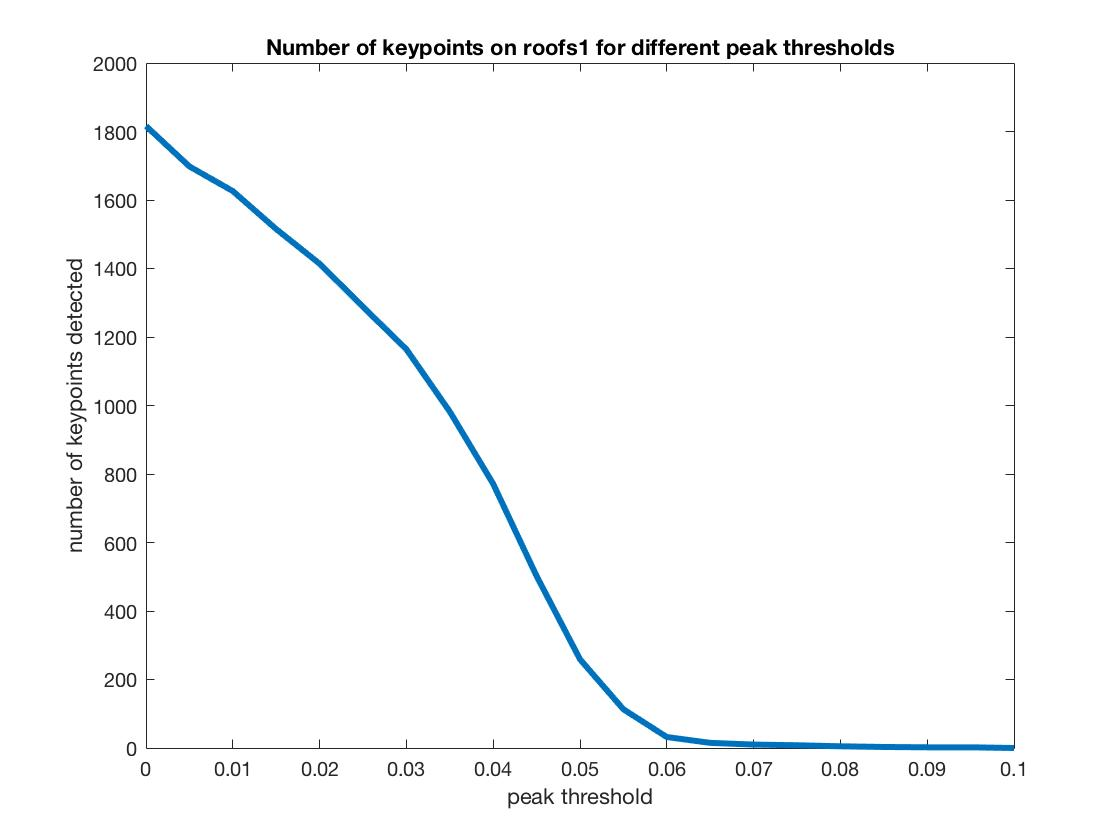
\includegraphics[width=\textwidth]{img/n_peak_thresh}
  \caption{Relationship between peak threshold and number of detected keypoints}
  \label{fig:n_peak_thresh}
\end{figure}

The number of detected keypoints decreases when increasing the threshold, since more and more keypoints with low extreme values of the difference of Gaussian in the scale space are filtered out, until finally there are none left. The peak threshold leads to the behavior we would expect. 

\begin{figure}[!hbt]
  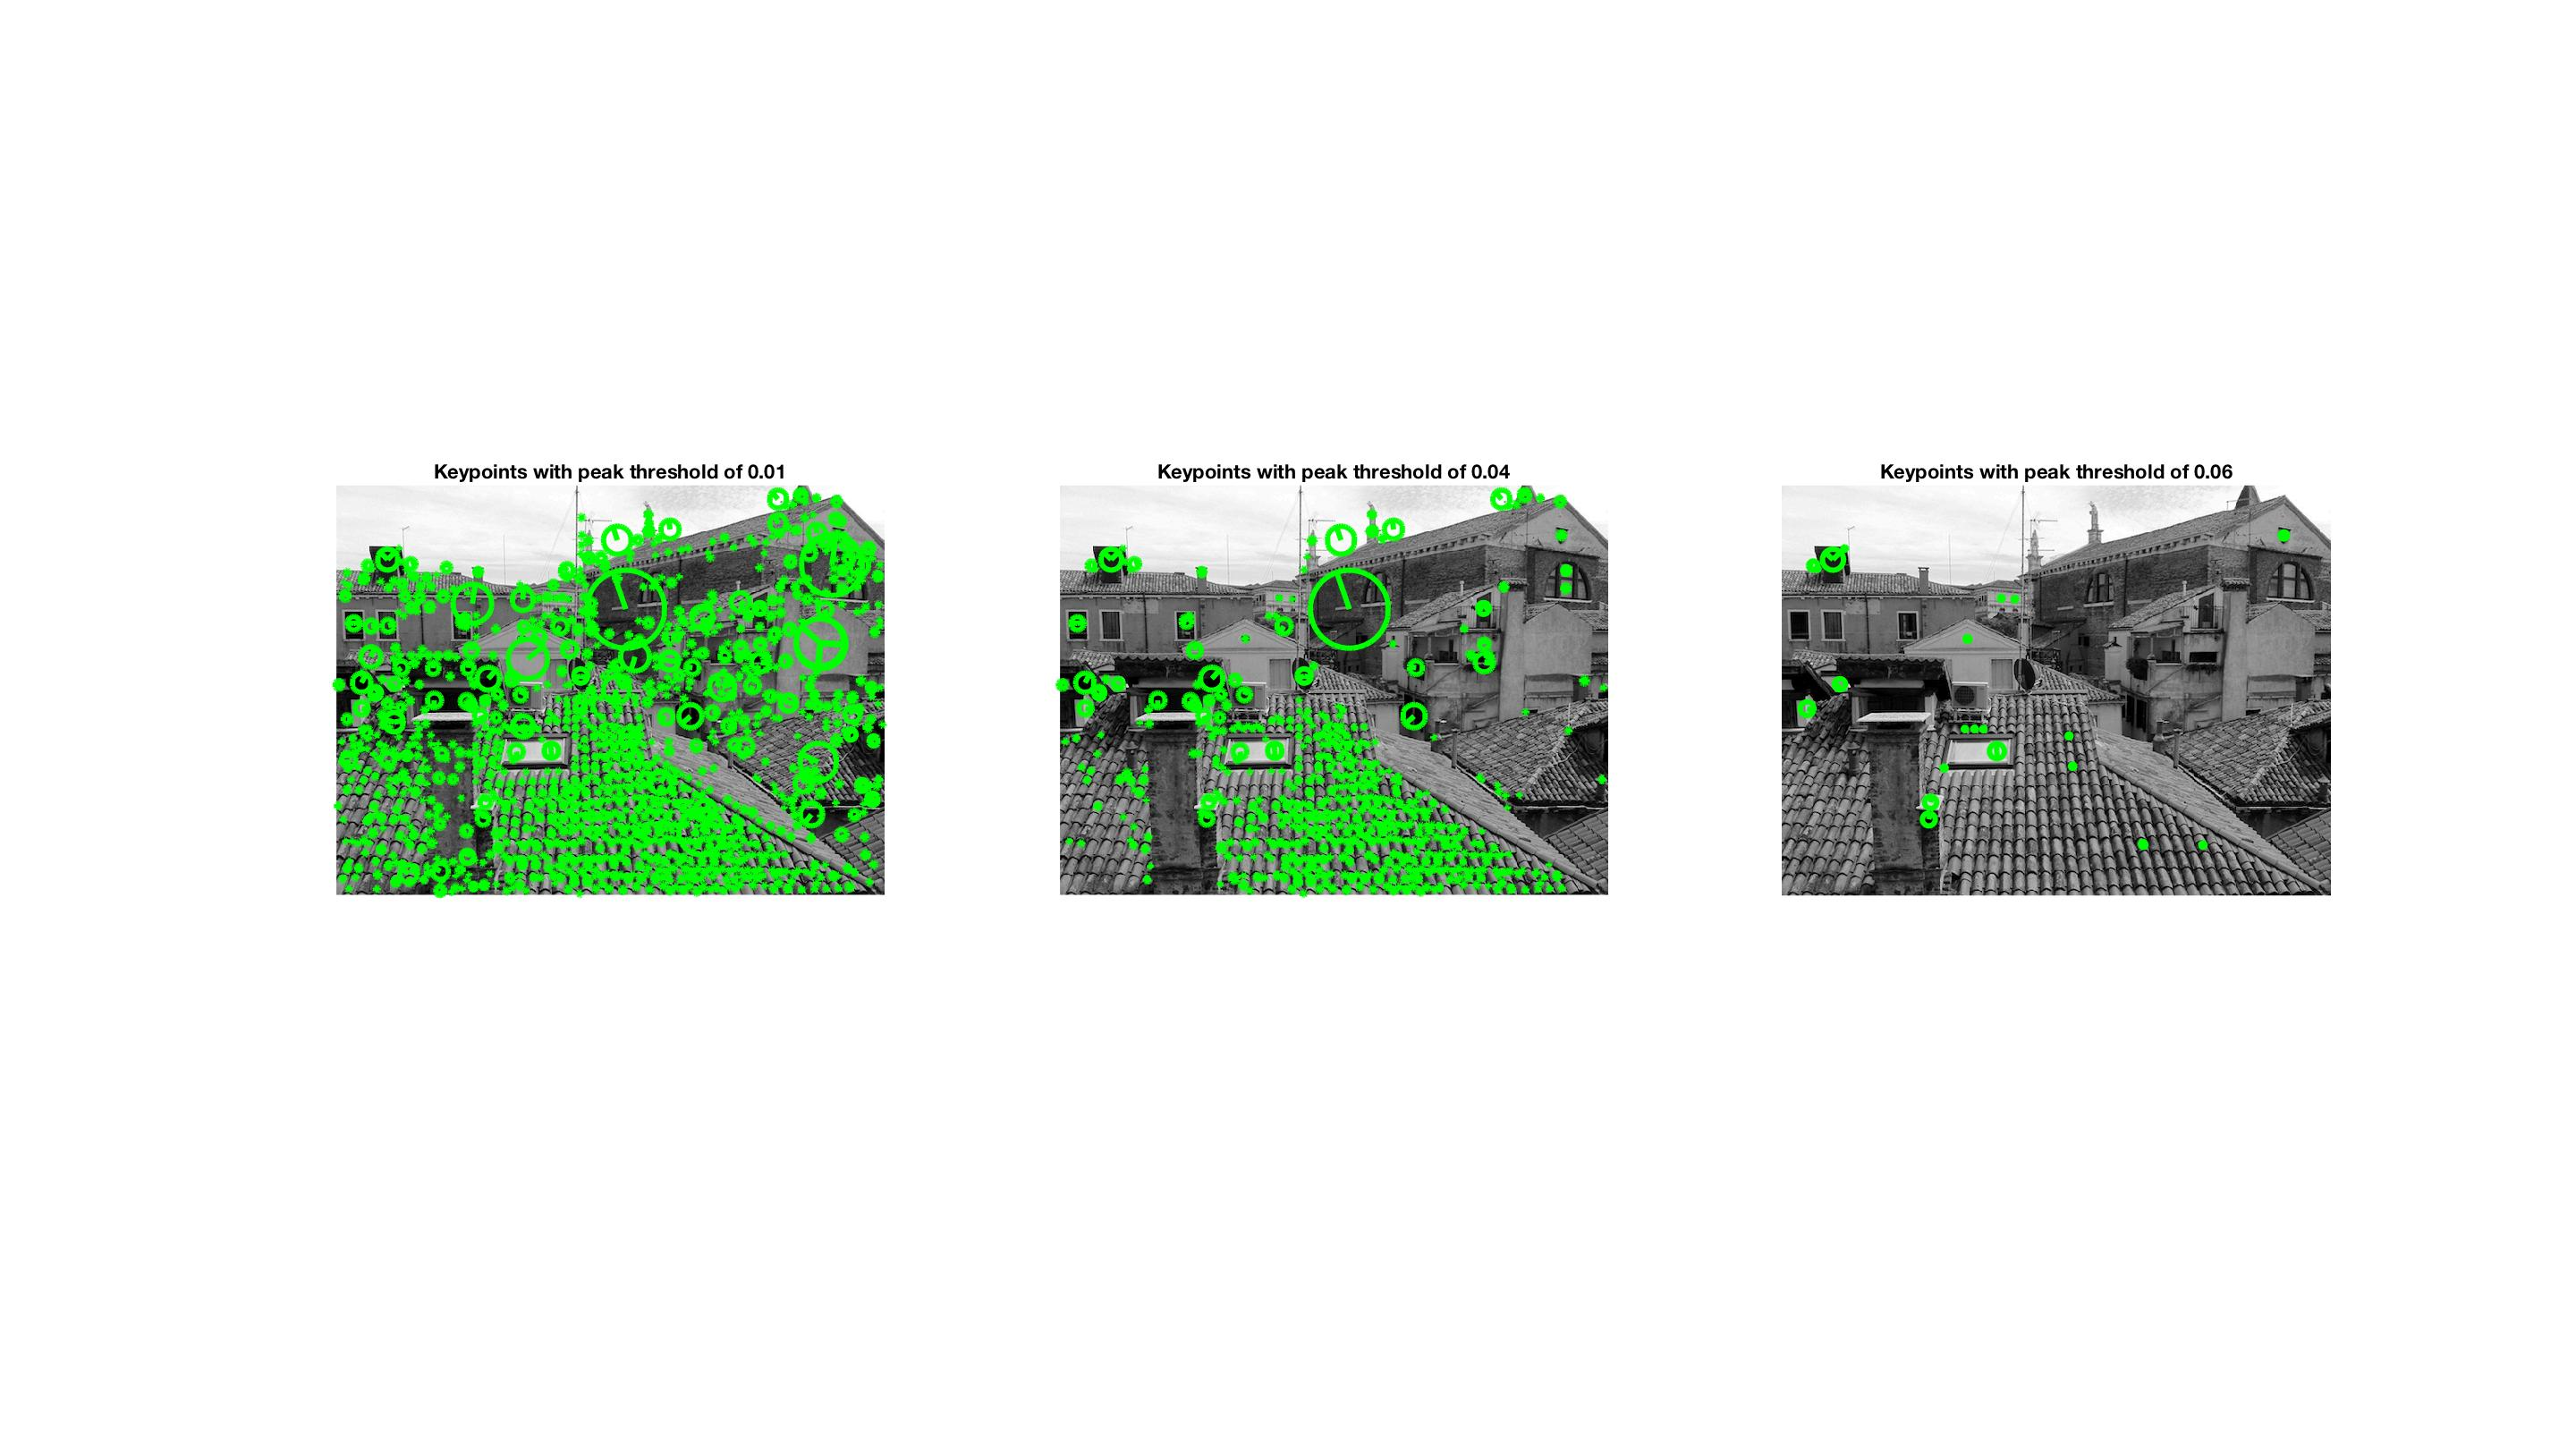
\includegraphics[width=\textwidth]{img/inc_peak_thresh}
  \caption{Effects of increasing the peak threshold}
  \label{fig:inc_peak_thresh}
\end{figure}

Figure \ref{fig:inc_peak_thresh} shows the effects of increasing the peak threshold on the example image \texttt{roofs1}. Keypoints in areas with low contrast and thus low extrema are sorted out first. For a threshold of 0.01 keypoints in the low contrast sky almost entirely are sorted out. For a threshold of 0.04, keypoints on the roof tiles begin to disappear. For a threshold of 0.06 only a few keypoints in very distinct positions remain.

\newpage